\chapter{Moving Relays}
\section{Mobility Model}
\subsection{Random Waypoint}

\section{Leaving in  one transition}
Let us find the probability with which a node at $(r,\theta)$ leaves the region in 
one transition. 
\subsection{Distances and Angles}
Consider the figure \ref{fig:rr1}. 
\begin{figure}[h]
    \centering \vspace{-0.1in}
    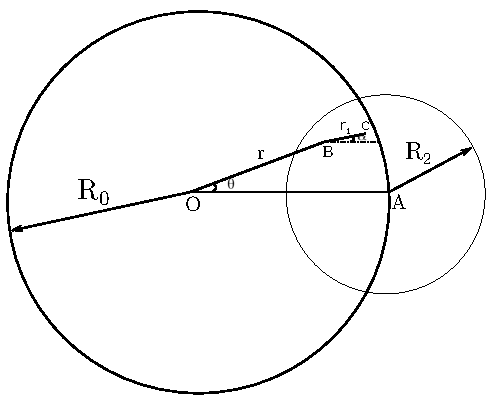
\includegraphics[width=0.6\textwidth]{images/geo1.pdf}
    \vspace{-20pt} \caption[Effect of the proximal Operator]{\small Effect of the Proximal Operator \footnotemark}
    \label{fig:rr1}
\end{figure}
\footnotetext{Image Source: \url{http://www.stanford.edu/~boyd/papers/pdf/prox_algs.pdf}}
The node starts at $B$ and let $C$ be 
the destination during first transition. $\alpha, r_1$ are chosen according to the mobility 
model described in the previous section. Whether or not $C$ is outside the region depends on
its distance from the circles' centers $O$ and $C$. $OC$ can be found using cosine rule:
$OC^2 = OB^2 + BC^2 - 2 \cdot OB \cdot BC \cdot \cos(\angle CBO)$. $\angle CBO = \pi-\theta+\alpha$ (see figure \ref{fig:ocac}).
\begin{figure}[h]
    \centering \vspace{-0.1in}
    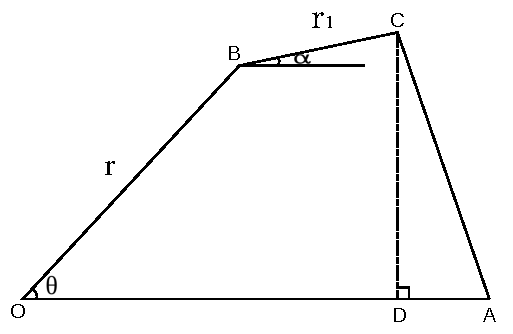
\includegraphics[width=0.6\textwidth]{images/geo2.pdf}
    \vspace{-20pt} \caption[Effect of the proximal Operator]{\small Effect of the Proximal Operator }
    \label{fig:ocac}
\end{figure}

 Therefore, \begin{equation} OC^2 = r^2 + r_1^2 + 2rr_1\cos(\theta-\alpha) \end{equation} To find $AC$, drop a perpendicular from $C$ to the line $OA$ and let the intersection point be $D$ as shown in figure \ref{fig:ocac}. Consider $\bigtriangleup CDA$, 
\begin{align*}
CD &= OB\sin\theta + BC\sin\alpha \\
&= r\sin\theta + r_1\sin\alpha \\
DA &= OA - OB\cos\theta - BC\cos\alpha \\
&= R_0-r\cos\theta-r_1cos\alpha
\end{align*}
Since $\angle CDA = \pi/2$, $AC^2 = CD^2 + DA^2$. $AC$ can therefore be given by 
\begin{equation}
	AC^2 = (r\sin\theta + r_1\sin\alpha)^2 + (R_0-r\cos\theta-r_1cos\alpha)^2
\end{equation}
To find which circle the node crosses first, we also need the angle made by the circle intersections at $B$. Let $\alpha_1$ and $\alpha_2$ be as shown in figures \ref{fig:alpha1} and \ref{fig:alpha2} where $BH$ is a horizontal line. 


\begin{figure}[h]
\centering \vspace{-0.1in}
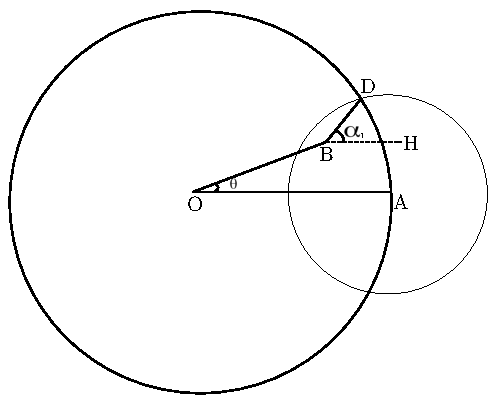
\includegraphics[width=0.6\textwidth]{images/geo3.pdf}
\vspace{-20pt} \caption[Effect of the proximal Operator]{\small Effect of the Proximal Operator }
\label{fig:alpha1}
\end{figure} 
\newpage
In figure \ref{fig:alpha1}, join $OD$ and drop
a perpendicular from $D$ to meet the extension of the $OB$ at $E$. To avoid clutter, let us 
remove the circles and form figure \ref{fig:alpha11}. 
\begin{figure}[h]
\centering \vspace{-0.1in}
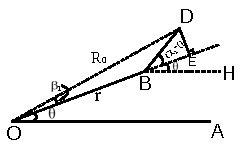
\includegraphics[width=0.6\textwidth]{images/geo4.pdf}
\vspace{-20pt} \caption[Effect of the proximal Operator]{\small Effect of the Proximal Operator }
\label{fig:alpha11}
\end{figure}
Consider $\bigtriangleup DOA$, 
\begin{align*}
	AD^2 &= OD^2 + OA^2 - 2 \cdot OD \cdot OA \cdot \cos(\beta_1+\theta) \\
	R_2^2 &= R_0^2 + R_0^2 - 2R_0^2\cos(\beta_1 + \theta)\\
\end{align*}
\begin{equation}\label{eq:beta1}
	\beta_1 = \cos^{-1}\bigg(1-\frac{R_2^2}{2R_0^2}\bigg) - \theta
\end{equation}
Using $\beta_1$ we can find $\alpha_1$
\begin{align*}
	\tan(\alpha_1 - \theta) &= \frac{DE}{BE} \\[2ex]
							&= \frac{DE}{OE-OB}\\[2ex]
							&= \frac{R_0 \sin\beta_1}{R_0\cos\beta_1 - r} \\[2ex]
	\alpha_1 &= \theta + \tan^{-1}\bigg( \frac{R_0 \sin\beta_1}{R_0\cos\beta_1 - r}\bigg) 
\end{align*}
\begin{figure}[h]
\centering \vspace{-0.1in}
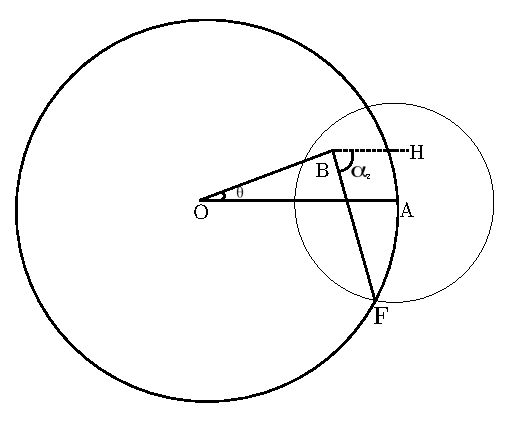
\includegraphics[width=0.6\textwidth]{images/geo5.pdf}
\vspace{-20pt} \caption[Effect of the proximal Operator]{\small Effect of the Proximal Operator }
\label{fig:alpha2}
\end{figure}
$\alpha_2$ and $\beta_2$ are defined in figures \ref{fig:alpha2} and \ref{fig:alpha21}. $\beta_2 = \beta_1 + \theta$ by symmetry. Using expression \ref{eq:beta1} for $\beta_1$, we get

\begin{equation}\label{eq:beta2}
	\beta_2 = \cos^{-1}\bigg(1-\frac{R_2^2}{2R_0^2}\bigg)
\end{equation}

\begin{figure}[h]
\centering \vspace{-0.1in}
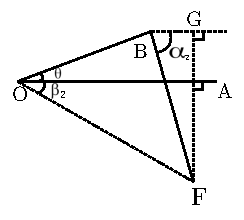
\includegraphics[width=0.6\textwidth]{images/geo6.pdf}
\vspace{-20pt} \caption[Effect of the proximal Operator]{\small Effect of the Proximal Operator }
\label{fig:alpha21}
\end{figure}

To find $\alpha_2$, consider $\bigtriangleup BGF$ in figure \ref{fig:alpha21}

\begin{align*}
	\tan\alpha_2 &= \frac{FG}{GB} \\[2ex]
			  &= \frac{FA+AG}{GB} \\[2ex]
			  &= \frac{R_0 \sin\beta_2 + r\sin\theta}{R_0 \cos\beta_2 - r\cos\theta} \\[2ex]
\Rightarrow \alpha_2 &= \tan^{-1}\bigg( \frac{R_0 \sin\beta_2 + r\sin\theta}{R_0 \cos\beta_2 - r\cos\theta} \bigg) 
\end{align*}

\subsection{Probability}
When $-\alpha_2 < \alpha < \alpha_1$, $C$ is outside the region if $OC^2 > R_0^2$ and for other values of $\alpha$, the node leaves the region if $AC^2 > R_2^2$. The probability of node leaving the region in one transition, let us call it $\rho(r,\theta)$
, is given by
\begin{equation}\label{eq:prob1}
	\rho(r,\theta) = Pr(-\alpha_2 < \alpha < \alpha_1,OC^2 > R_0^2) + Pr(\alpha_1 < \alpha < 2\pi-\alpha_2, AC^2 > R_2^2) \\
\end{equation}
Let us rewrite the above in terms of $r_1$ whose distribution we know.
$AC^2 > R_2^2 \Rightarrow$

\begin{align*}
	(r\sin\theta + r_1\sin\alpha)^2 + (R_0-r\cos\theta-r_1cos\alpha)^2 &> R_2^2 \\
	r_1^2 \sin^2\alpha + r^2\sin^2\theta + 2rr_1\sin\theta\sin\alpha &+ \\ (R_0-r\cos\theta)^2 +
	r_1^2\cos^2\alpha - 2(R_0-r\cos\theta)r_1\cos\alpha - R_2^2 &> 0\\ 
	r_1^2 + 2 r_1 (r\sin\alpha\sin\theta-(R_0-r\cos\theta)\cos\alpha) + r^2\sin^2\theta +
	(R_0-r\cos\theta)^2 -R_2^2 &>0 \\
	r_1^2 + 2(r\cos(\theta-\alpha) - R_0\cos\alpha) r_1 + r^2\sin^2\theta +	(R_0-r\cos\theta)^2 - R_2^2 &> 0 
\end{align*}
The above inequality gives two feasible intervals for $r_1$ one of which is spurious since $r_1 > 0$ and the other is 
\begin{align}\label{ineq:ACcon}
	r_1 > (R_0\cos\alpha - r\cos(\theta-\alpha)) + \sqrt{\big(R_0\cos\alpha-r\cos(\theta-\alpha)\big)^2 + R_2^2 - r^2\sin^2\theta - 	(R_0-r\cos\theta)^2 }
\end{align}
Similar calculations as above will reduce $OC^2 > R_0^2$ to
\begin{align} \label{ineq:OCcon}
	r_1 > -r\cos(\theta-\alpha) + \sqrt{R_0^2 - r^2\sin^2(\theta-\alpha)}
\end{align}
Let us denote the R.H.S of the above two inequalities by $r_{12}$ and $r_{11}$ respectively.
Substituting \ref{ineq:ACcon} and \ref{ineq:OCcon} in \ref{eq:prob1}, we get
\begin{align*}
	\rho(r,\theta) &= Pr(-\alpha_2 < \alpha < \alpha_1,r_1 > r_{11}) + Pr(\alpha_1 < \alpha < 2\pi-\alpha_2, r_1 > r_{12}) \\
	&= \int_{-\alpha_2}^{\alpha_1} \int_{r_{\!_{11}}}^{\infty} f_{r_1,\alpha}(r_1,\alpha)dr_1 d\alpha +  \int^{2\pi-\alpha_2}_{\alpha_1} \int_{r_{\!_{12}}}^{\infty} f_{r_1,\alpha}(r_1,\alpha)dr_1 d\alpha 
\end{align*}
	This is a general expresion that can be used for any mobility model. In case of RWP,
	$r_1$ and $\alpha$ are chosen independently. Therefore, 
	$f_{r_1,\alpha}(r_1,\alpha) = f_{r_1}(r_1)f_{\alpha}(\alpha)$ 
\begin{align*}
	\rho(r,\theta)&= \int_{-\alpha_2}^{\alpha_1} f_{\alpha}(\alpha) \int_{r_{\!_{11}}}^{\infty} f_{r_1}(r_1)dr_1 d\alpha +  \int^{2\pi-\alpha_2}_{\alpha_1} f_{\alpha}(\alpha) \int_{r_{\!_{12}}}^{\infty} f_{r_1}(r_1)dr_1 d\alpha  \\
	&= \int_{-\alpha_2}^{\alpha_1} \frac{1}{2\pi} e^{-\lambda \pi r_{\!_{11}}^2} d\alpha +  \int^{2\pi-\alpha_2}_{\alpha_1} \frac{1}{2\pi} e^{-\lambda \pi r_{\!_{12}}^2} d\alpha
\end{align*}
\newpage
Putting it all together at one place for ease of reference, this is what have about the node's
first transition. \\
The probability with which a 
node at $(r,\theta)$ moves out of the region of interest during the next transition is 
\begin{equation} \label{eq:oneOutProb}
	\rho(r,\theta) = \int_{-\alpha_2}^{\alpha_1} \frac{1}{2\pi} e^{-\lambda \pi r_{\!_{11}}^2} d\alpha +  \int^{2\pi-\alpha_2}_{\alpha_1} \frac{1}{2\pi} e^{-\lambda \pi r_{\!_{12}}^2} d\alpha
\end{equation}
\\
Where
\begin{align*}
	r_{\!_{11}} &= -r\cos(\theta -\alpha) + \sqrt{R_0^2 - r^2\sin^2(\theta - \alpha)} \\
	&\\
	r_{\!_{12}} &= R_0 \cos \alpha - r\cos(\theta - \alpha)  +  \sqrt{[R_0 \cos \alpha - r\cos(\theta-\alpha) ]^2 - r^2\sin^2 \theta - [R_0 - r\cos \theta]^2 + R_2^2} \\
\end{align*}
\begin{align*}
	\beta_1 &= \cos^{-1}\bigg(1-\frac{R_2^2}{2R_0^2}\bigg) - \theta \\
	& \\
		\beta_2 &= \cos^{-1}\bigg(1-\frac{R_2^2}{2R_0^2}\bigg) \\
	& \\
	\alpha_1 &= \theta + \tan^{-1}\bigg( \frac{R_0\sin\beta_1}{R_0\cos\beta_1-r}\bigg)\\
			& \\
			\alpha_2 &= \tan^{-1}\bigg( \frac{r\sin\theta + R_0\sin\beta_2}{R_0cos\beta_2 - r\cos\theta} \bigg)
\end{align*}
